% !TEX program = xelatex

\documentclass[11pt, article, natbib]{IEEEtran}
% \IEEEoverridecommandlockouts
\usepackage[utf8]{inputenc}
\usepackage[spanish]{babel}
\usepackage{fancyhdr}
\usepackage{mathtools}
\usepackage{tikz}
\usepackage{setspace}
% \usepackage{apacite}
\usepackage[backend=biber, style=apa]{biblatex}
\addbibresource{ref.bib}

\pagestyle{fancy}
\fancyhf{Universidad Nacional de Costa Rica}
\rhead{\thepage}
\lhead{Investigación \# 4}
\rfoot{EIF-402 Bases de Datos II}
\lfoot{II-2023}

\def\changemargin#1#2{\list{}{\rightmargin#2\leftmargin#1}\item[]}
\let\endchangemargin=\endlist

\DeclarePairedDelimiter\ceil{\lceil}{\rceil}
\DeclarePairedDelimiter\floor{\lfloor}{\rfloor}
\makeatletter
\renewcommand*\l@section{\@dottedtocline{1}{1.5em}{2.3em}}
\makeatother

\begin{document}

\begin{titlepage}
	
\includegraphics[width=0.2\textwidth]{../../../Files/logo-UNA blanco.png}
    \vspace{1cm}
   	\begin{changemargin}{4.5cm}{0cm}
       	\textbf{\Huge Estrategia de recuperación de base de datos}

       	\vspace{0.2cm}
       	\LARGE Tarea Investigación \# 4
            
       	\vspace{2cm}
		\Large
        Yiriana Georgeth Guevara Araya \\
        Jorge Andrés Durán Campos \\
        Luis Antonio Montes de Oca Ruiz \\
       	Diego Quirós Artiñano \\ 

       	\vspace{2cm}
       
		EIF-402 Administración de bases de datos \\
       	Profesor Johnny Villalobos Murillo \\
		       	
       	\vfill


       	\today
	\end{changemargin}
\end{titlepage}

\onecolumn
% Índices
\pagenumbering{roman}
    % Contenido
    \renewcommand{\contentsname}{\large Índice \\ \hrulefill}
\tableofcontents
\setcounter{tocdepth}{2}

\newpage
%     Figuras
%  \renewcommand{\listfigurename}{\large Índice de fíguras \\ \hrulefill}
%  \listoffigures
%  \newpage
     % Tablas
%  \renewcommand{\listtablename}{\large Índice de tablas \\ \hrulefill}
%  \listoftables
%  \newpage
% Cuerpo
\pagenumbering{arabic}

\twocolumn
\onehalfspace
\section{Diagnóstico (Parte 19 de octubre, 2023)}
Lista de errores que estaban en la base de datos:
\begin{itemize}
	\item Falta de archivo de la base de datos (.dbf)
	\item Falta de archivo de control (.ctl)
\end{itemize}

Al intentar hacer una petición cualquiera desde el usuario system presenta el siguiente error.

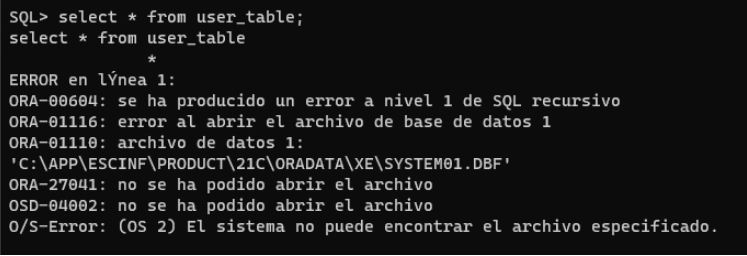
\includegraphics[width=0.4\textwidth]{./images/image1diag.png}

Este error implica que se perdió el archivo de base de datos por lo cual ya no se puede abrir

Además intentando de revisar el último log no logra encontrar el archivo de control file indicado por el siguiente error.

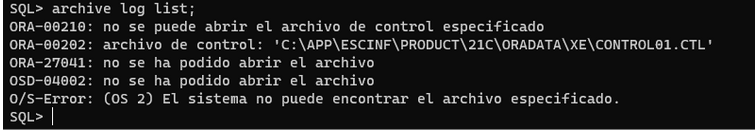
\includegraphics[width=0.4\textwidth]{./images/image2diag.png}

Igualmente la base de datos parece no tener logs por lo que se puede ver en la siguiente dirección: \textit{'C:\textbackslash app\textbackslash ESCINF\textbackslash product\textbackslash 21c\textbackslash homes\textbackslash OraDB21Hom\\e1\textbackslash rdbms'}

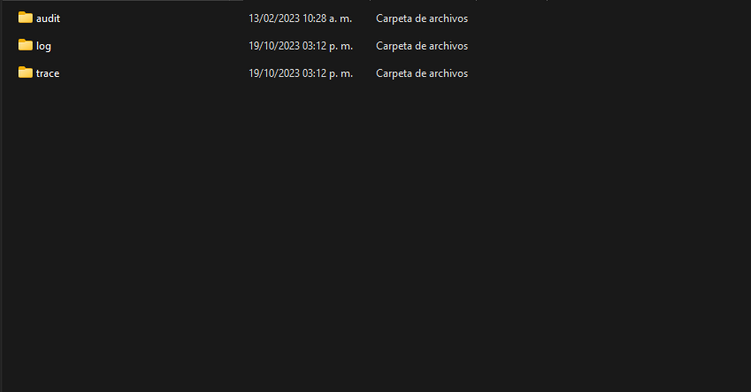
\includegraphics[width=0.4\textwidth]{./images/image3diag.png}

Esto no es indicatorio y sin el control file no se puede saber la dirección real que se está utilizando, pero según la dirección por defecto ese debería ser.

No es un error pero hace falta recalcar: como se logra ingeresar a las base de datos entonces se sabe que el innit existe y no está dañado, esto se puede corroborar por los siguientes archivos

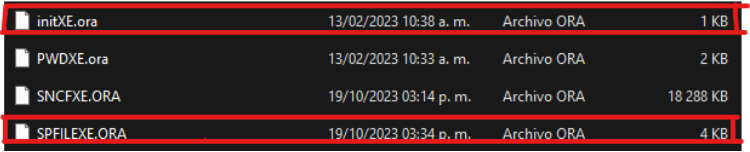
\includegraphics[width=0.4\textwidth]{./images/image4diag.png}

Esos archivos se ubican en la dirección: \textit{'C:\textbackslash app\textbackslash ESCINF\textbackslash product\textbackslash 21c\textbackslash database'}
% \newpage
% \twocolumn
\section{Estretegia para recuperar .ctl}
Note que si lo que falta es el spfile se tiene que recuperar eso primero.

Sin los controlfiles rman no puede funcionar correctamente por lo cual es lo primero que se tiene que mandar a recuperar.

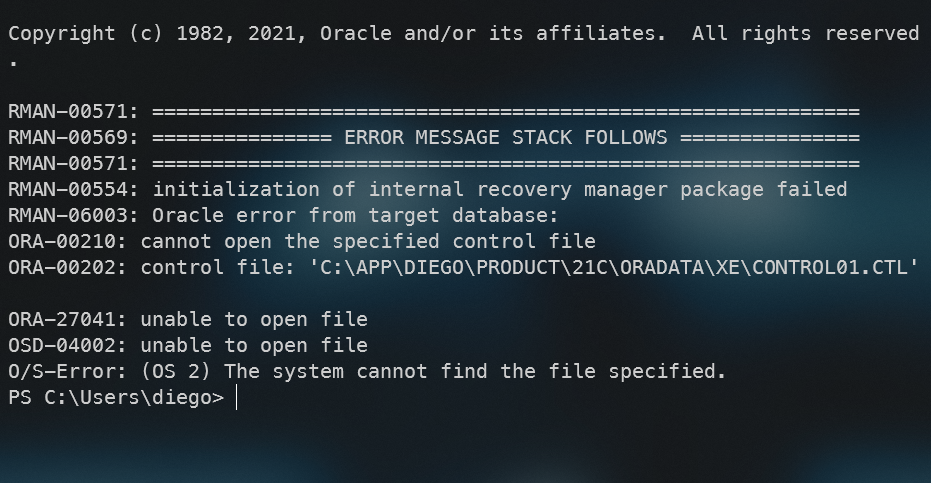
\includegraphics[width=0.4\textwidth]{./images/RMANERROR.png}

Para poder recuperar la base de datos hay que hacerle \textit{shutdown abort;} a la base de datos.


\includegraphics[width=0.4\textwidth]{./images/shutdown.png}

Después se ingresa a RMAN y se setea el DBID con los comandos:
\textit{rman target /} y \textit{set DBID <número que aparece cuando ingresas a RMAN normalmente>;}

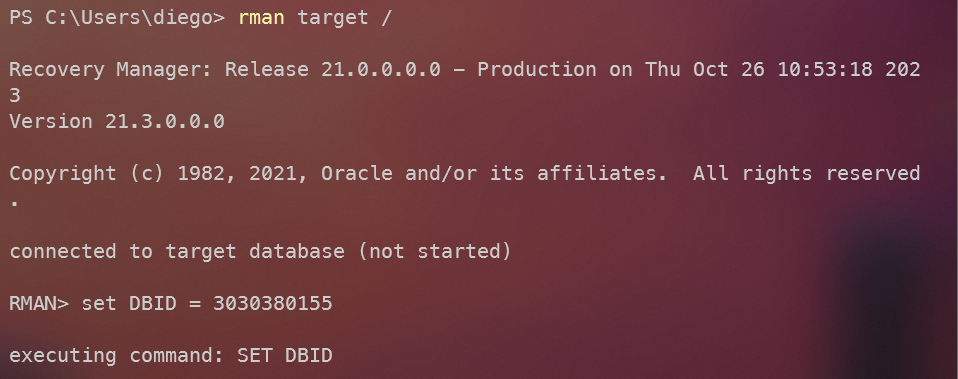
\includegraphics[width=0.4\textwidth]{./images/setDBID.png}

La imagen anterior muestra como se ve durante la recuperación

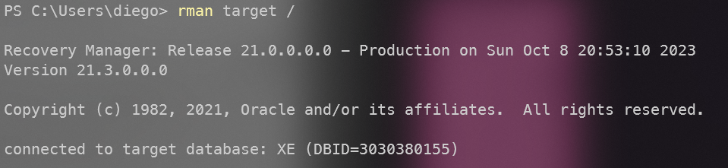
\includegraphics[width=0.4\textwidth]{./images/DBID.png}

La imagen anterior muestra como se debería ver normalmente y el DBID al que se tiene que setear para recuperar la base de datos.

Después se le hace \textit{startup nomount;} para ingresar a la base de datos y después se puede hacer \textit{restore controlfile from <nombre de archivo guardado>;}. Notese que en la imagen se pone autobackup, porque al hacer el fullbackup el RMAN que se tenía configurado hacía el backup del controlfile, si no se tiene activado esto se tiene que hacer el backup manualmente.

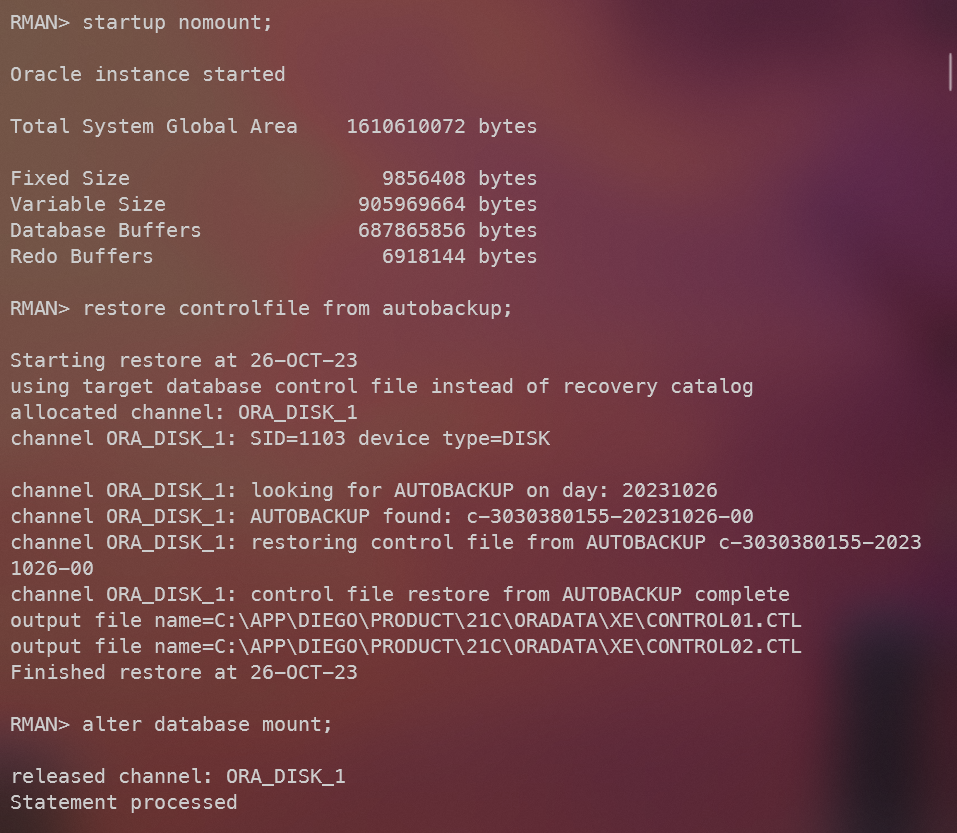
\includegraphics[width=0.4\textwidth]{./images/restoreControlfile.png}

de una vez se puede hacerle \textit{restore archivelog all;} para recuperar los archivelogs

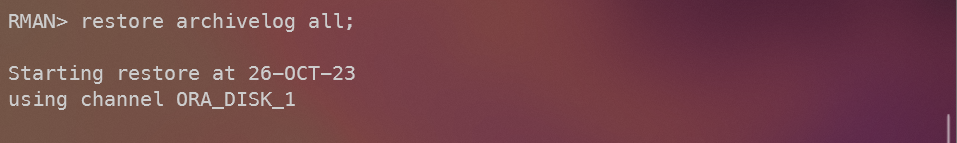
\includegraphics[width=0.4\textwidth]{./images/restoreArchvieLog.png}

Así ya se tiene hecho el restore de los controlfiles y se puede continuar a la base de datos.

\section{Estrategia para recuperar .dbf}

Para lo siguiente primero es bueno validar los backups que se tienen hasta el momento, para esto primero revisar los backups con \textit{restore database summary preview;}

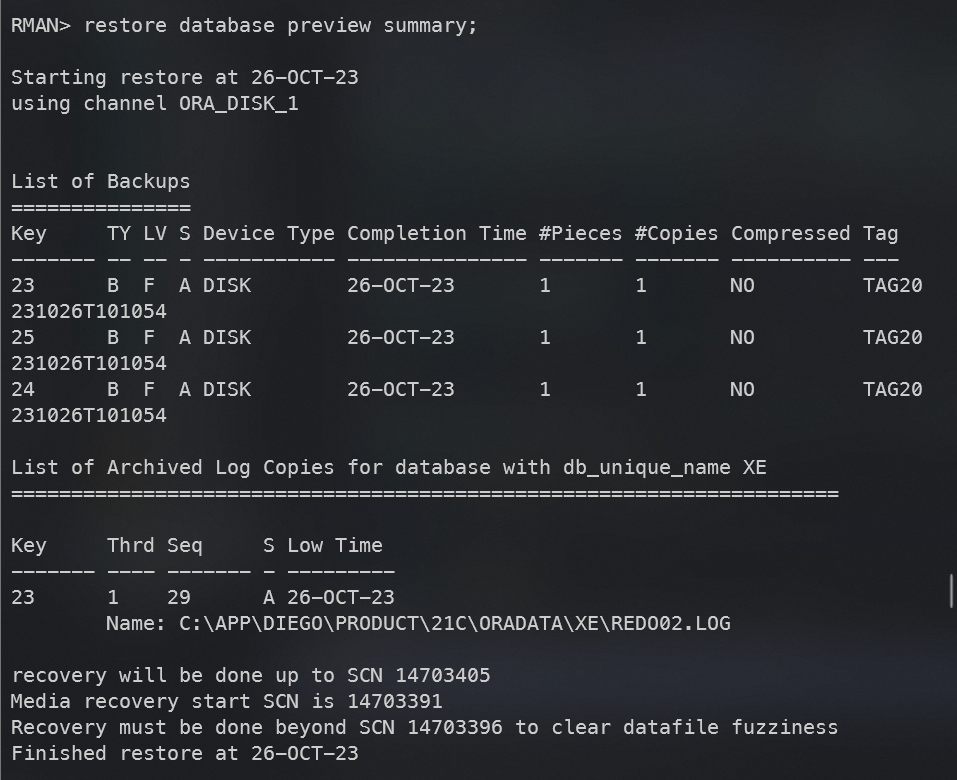
\includegraphics[width=0.4\textwidth]{./images/restoreDatabasePreviewSummary.png}

Después se sigue la validación con el comando \textit{validate backupset <numero del backupset mostrado por el database summary>;}

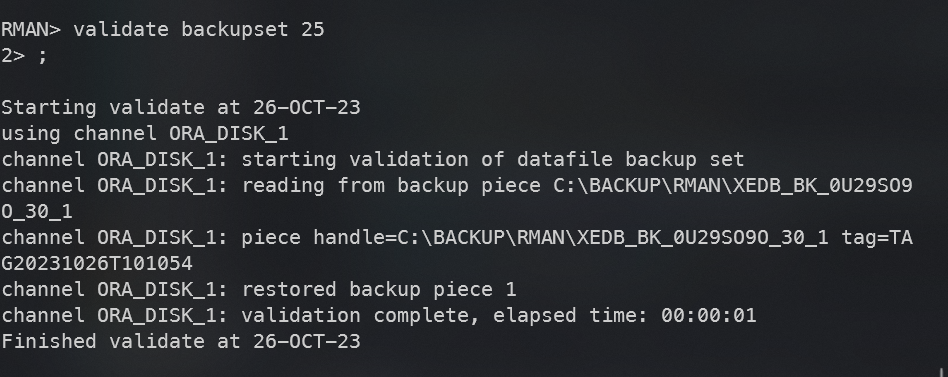
\includegraphics[width=0.4\textwidth]{./images/validateBackupset.png}

Finalmente, se puede ejecutar los comandos de \textit{restore database;} y \textit{recover database;} seguidos.

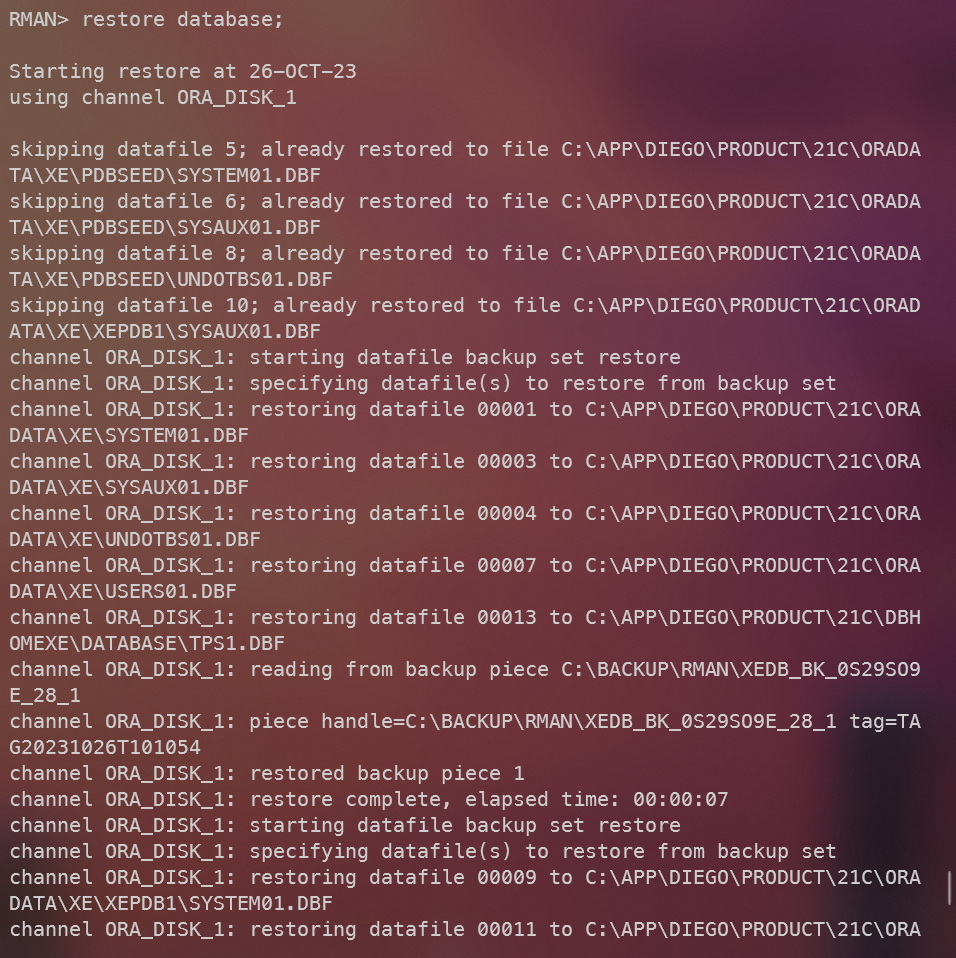
\includegraphics[width=0.4\textwidth]{./images/restoreDatabase.png}

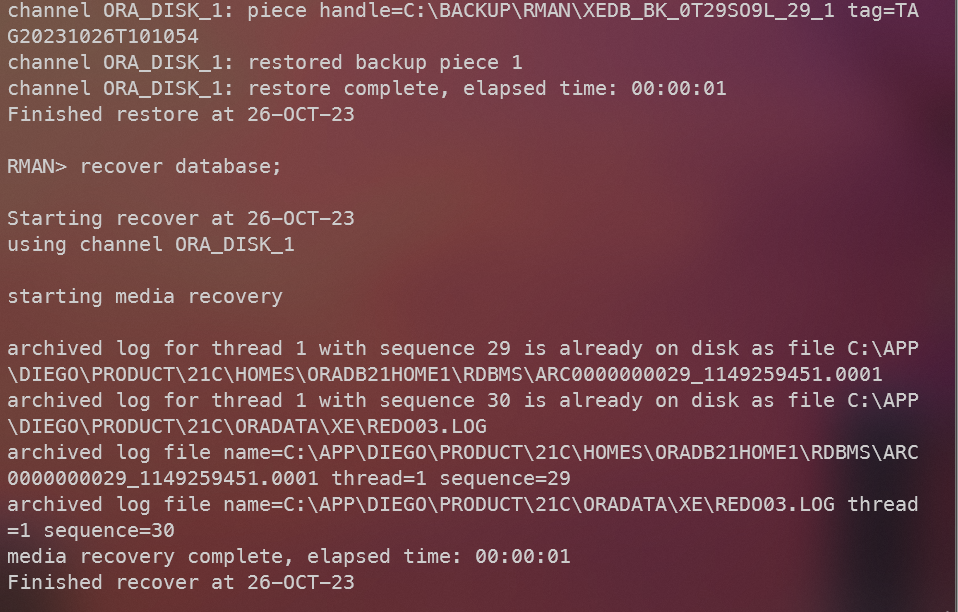
\includegraphics[width=0.4\textwidth]{./images/recoverDatabase.png}

\newpage
\onecolumn


\nocite{errorLoginRMAN}
\nocite{vinchin}
\nocite{wordpress}
\nocite{oracleSupport}
\nocite{oracleDocs}
% \bibliographystyle{apa} 
% \bibliography{ref.bib}
\printbibliography

\end{document}